\documentclass[12pt]{article}
\usepackage{amsmath, amssymb}
\usepackage[margin=1.7cm]{geometry}
\usepackage{hyperref}
\usepackage{graphicx}
\usepackage{tikz}
\usepackage{enumitem}
\setlength{\parindent}{0pt}
\setlist{itemsep=0.35em, topsep=0.35em}

\title{Probearbeit 4}
\author{}
\date{07.12.2025}

\begin{document}
\maketitle

\textbf{PQ-Formel} für \(x^{2} + px + q = 0\):
\[
  x_{1,2} = -\frac{p}{2} \pm \sqrt{\left(\frac{p}{2}\right)^{2} - q}.
\]
Schreibe immer zuerst \(p\) und \(q\) auf, setze sie ein und berechne die Diskriminante. Exakte Werte reichen; nicht runden.

\section*{Aufgabe 1: Tabelle, Skizze, Nullstellen}
Betrachte \(f(x) = -x^{2} + 4x + 3\).
\begin{enumerate}
  \item Berechne \(f(x)\) für \(x = 0, 1, 2, 3, 4, 5\) und trage die Werte ein.
  \item Skizziere die Parabel mithilfe der Tabelle im Koordinatensystem. Markiere Scheitelpunkt (abgelesen aus der Skizze) und Symmetrieachse.
  \item Berechne die Nullstellen mit der PQ-Formel. Tipp: Stelle \( -x^{2} + 4x + 3 = 0\) um zu \(x^{2} - 4x - 3 = 0\) und setze \(p = -4, \; q = -3\).
\end{enumerate}

\begin{center}
\begingroup
\renewcommand{\arraystretch}{1.8}
\begin{tabular}{|c|c|c|c|c|c|c|}
  \hline
  \(x\) & \(0\) & \(1\) & \(2\) & \(3\) & \(4\) & \(5\) \\
  \hline
  \(y = f(x)\) & & & & & & \\
  \hline
\end{tabular}
\endgroup
\end{center}

\begin{center}
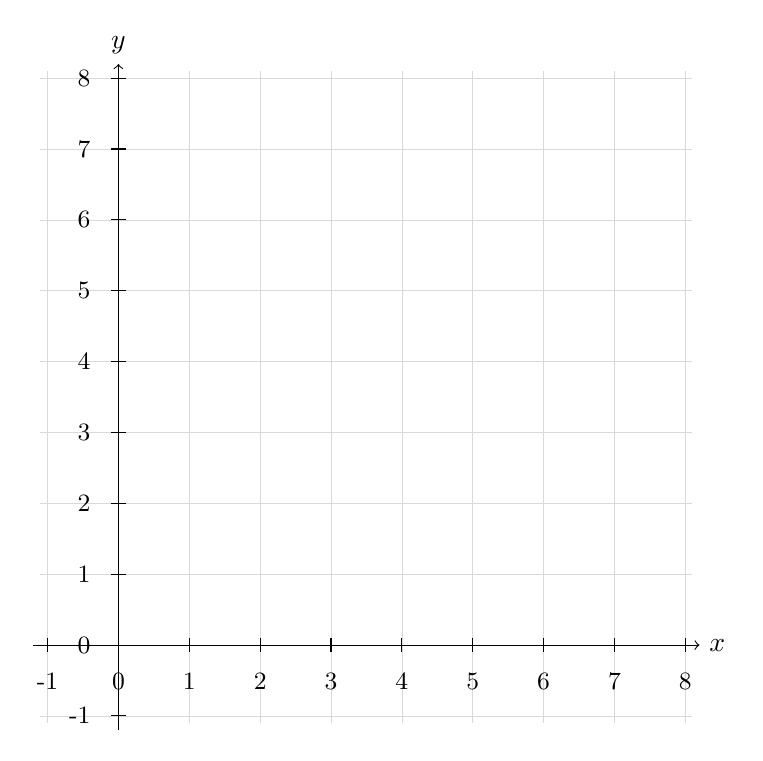
\begin{tikzpicture}[scale=0.9]
  \draw[step=1cm,gray!30,very thin] (-1.1,-1.1) grid (8.1,8.1);
  \draw[->] (-1.2,0) -- (8.2,0) node[right] {$x$};
  \draw[->] (0,-1.2) -- (0,8.2) node[above] {$y$};
  \foreach \x in {-1,0,...,8} \draw (\x,0.1) -- (\x,-0.1) node[below=4pt] {\small \x};
  \foreach \y in {-1,0,...,8} \draw (0.1,\y) -- (-0.1,\y) node[left=4pt] {\small \y};
\end{tikzpicture}
\end{center}


\section*{Aufgabe 3: Erst normieren, dann lösen}
Bringe jede Gleichung zuerst in die Form \(x^{2} + px + q = 0\), dann PQ-Formel.
\begin{enumerate}
  \item \(-2x^{2} + 8x - 6 = 0\)
  \item \(3x^{2} + 9x - 18 = 0\)
  \item \(5x^{2} - 10x - 15 = 0\)
\end{enumerate}

\section*{Aufgabe 4: Bonus -- Textaufgabe}
Eine Rakete wird von einer Startrampe abgeworfen. Ihre Höhe über dem Boden (in Metern) wird modelliert durch
\[
  h(t) = -5t^{2} + 20t + 5 \quad (t \text{ in Sekunden}).
\]
\begin{enumerate}
  \item Bestimme die Zeitpunkte, zu denen die Rakete den Boden erreicht (\(h(t) = 0\)). Tipp: Teile durch \(-5\), dann PQ.
  \item Wie lange bleibt die Rakete mindestens in der Luft? (Zeitspanne zwischen den beiden Nullstellen.)
  \item Berechne den Zeitpunkt der maximalen Höhe (Scheitelpunkt aus der Symmetrie zwischen den Nullstellen; kein Ableiten nötig).
\end{enumerate}

\end{document}
